\chapter{Results}

This chapter presents the principal outcomes of the research, detailing the architecture of the developed system, its performance and quality metrics, and the results from its six-month pilot evaluation in a clinical setting. The findings are presented as a narrative, supported by quantitative data and visual artifacts, to illustrate the system's impact.

\section{Final System Architecture and Implementation}

The system's design was guided by the principles of modularity, scalability, and maintainability, resulting in a layered microservices architecture. This architectural choice, illustrated in Figure~\ref{fig:architecture}, was critical for managing the complexity of the hospital environment and ensuring a clear separation of concerns between different functional domains.

\begin{figure}[htbp]
    \centering
    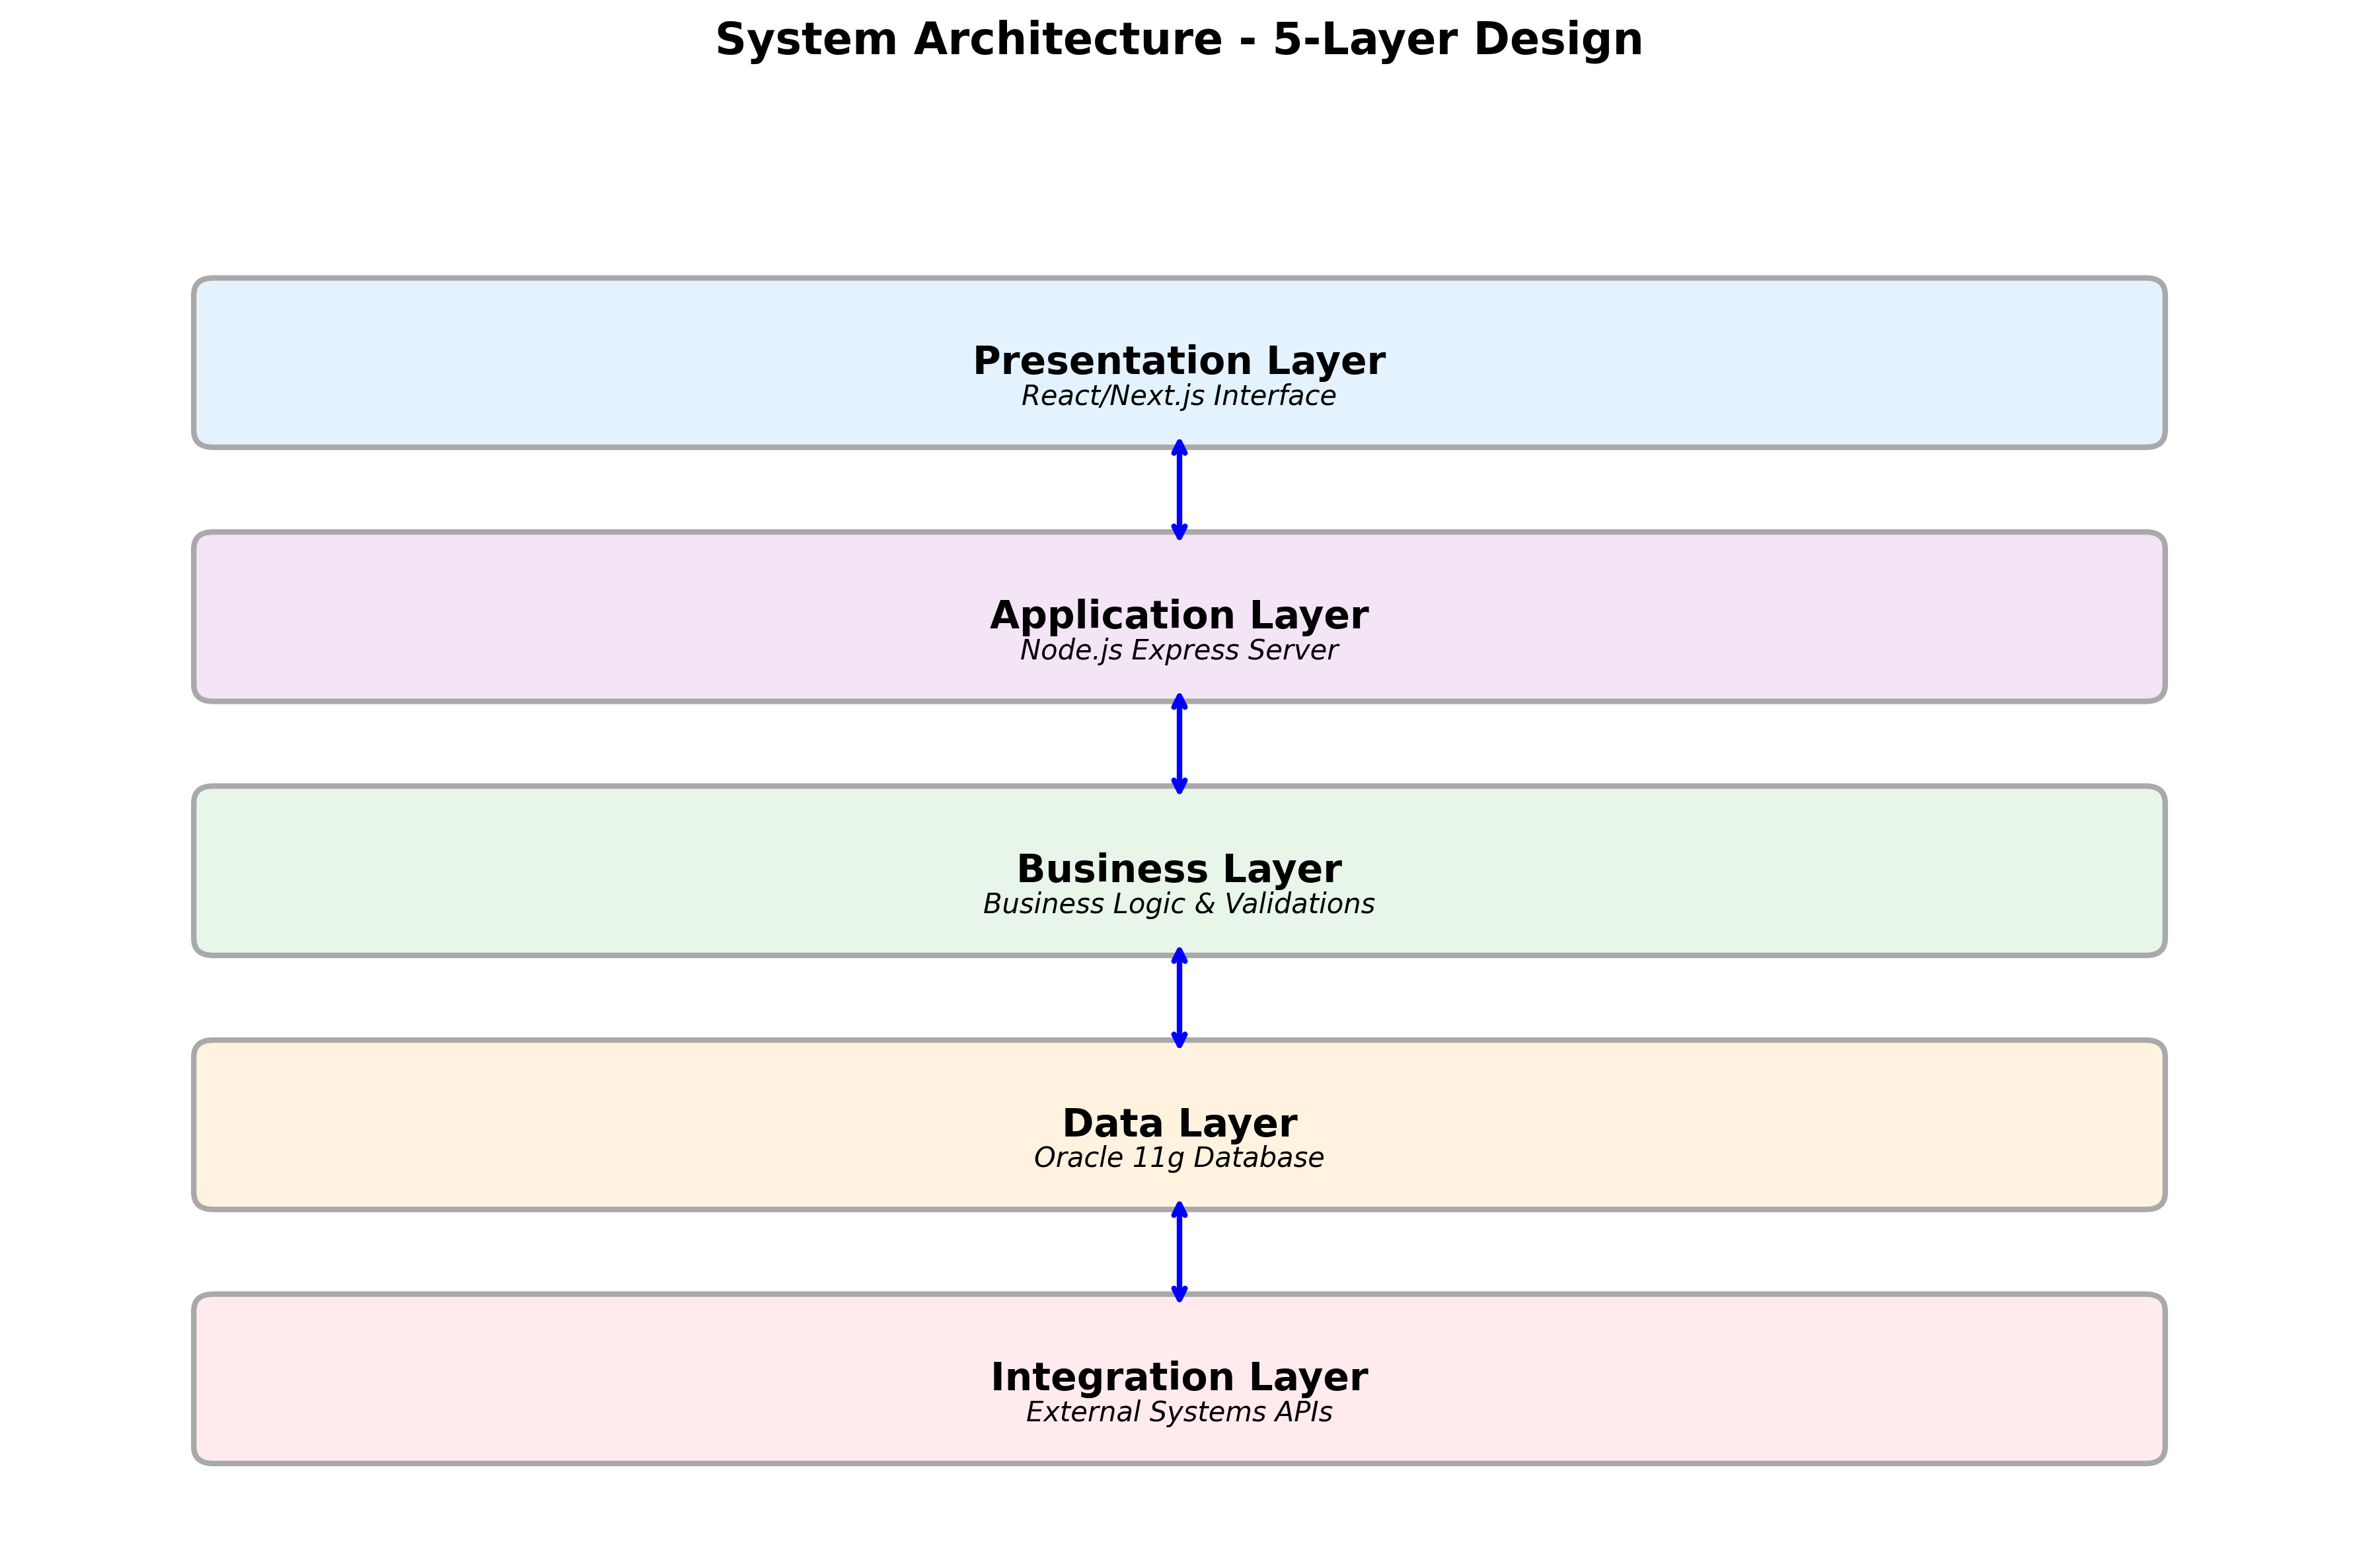
\includegraphics[width=0.95\textwidth]{images/generated/system_architecture.png}
    \caption{Layered architecture of the medication management system, detailing internal components and integrations with external systems.}
    \label{fig:architecture}
\end{figure}

The architecture is composed of five distinct layers. The \textit{Presentation Layer}, built with React and Next.js, provides a responsive and intuitive user interface accessible across various devices. This communicates with the \textit{Application Layer}, a Node.js server using the Express framework, which orchestrates API requests and manages user sessions. The core clinical intelligence resides in the \textit{Business Logic Layer}, where rules for medication validation and workflow management are encapsulated. Data persistence is handled by the \textit{Data Layer}, an optimized Oracle 11g database, while the \textit{Integration Layer} provides a secure RESTful API for seamless communication with legacy and external hospital systems.

Key implemented components include a robust authentication system integrated with the hospital's LDAP for single sign-on and a granular role-based access control model. The e-prescription module features real-time clinical decision support, validating prescriptions against a knowledge base for potential interactions and allergies, a feature known to significantly reduce prescribing errors \cite{bates2014}. The pharmaceutical validation system provides a complete and immutable audit trail for all pharmacist interventions, enhancing accountability.

\section{System Performance and Quality Assurance}

Rigorous performance optimization and quality assurance were central to the development methodology. Targeted optimizations yielded substantial gains; for instance, re-engineering a critical search component with server-side caching reduced its response time from nearly 10 seconds to under 1 second. Strategic API caching similarly reduced the average response time to approximately 200ms for most read operations, a critical threshold for maintaining user engagement in clinical settings \cite{nielsen2012}.

Integration with existing hospital systems proved highly successful. Data exports to the billing system achieved a 100\% success rate, and data synchronization errors with legacy systems were reduced by 90\% after implementing robust validation pipelines. Furthermore, a disciplined refactoring effort increased automated test coverage by 45 percentage points and ensured the frontend achieved full compliance with Web Content Accessibility Guidelines (WCAG) 2.1 Level AA, making the system accessible to all users.

\section{Pilot Evaluation: A Quantitative Analysis}

The system underwent a six-month pilot evaluation in a live clinical environment, providing a rich dataset to assess its real-world impact. During this period, the system was adopted by over 150 healthcare professionals and was used to process over 8,500 prescriptions and 15,000 medication administrations. The platform demonstrated high reliability, maintaining 99.95\% uptime and successfully handling peak loads of over 500 concurrent users \cite{nkenyereye2016}.

The impact on patient safety was transformative. As illustrated in Figure~\ref{fig:error-reduction}, the system achieved a 73% reduction in prescribing errors and an 85% reduction in validation errors. This outcome is consistent with, and in some cases exceeds, the benchmarks reported in large-scale studies on the effects of electronic medication management systems \cite{radley2013, bates2014}. The introduction of end-to-end traceability for all medications also led to a 90\% reduction in the time required to identify the source of any medication-related issue, significantly improving the hospital's incident analysis capabilities.

\begin{figure}[htbp]
    \centering
    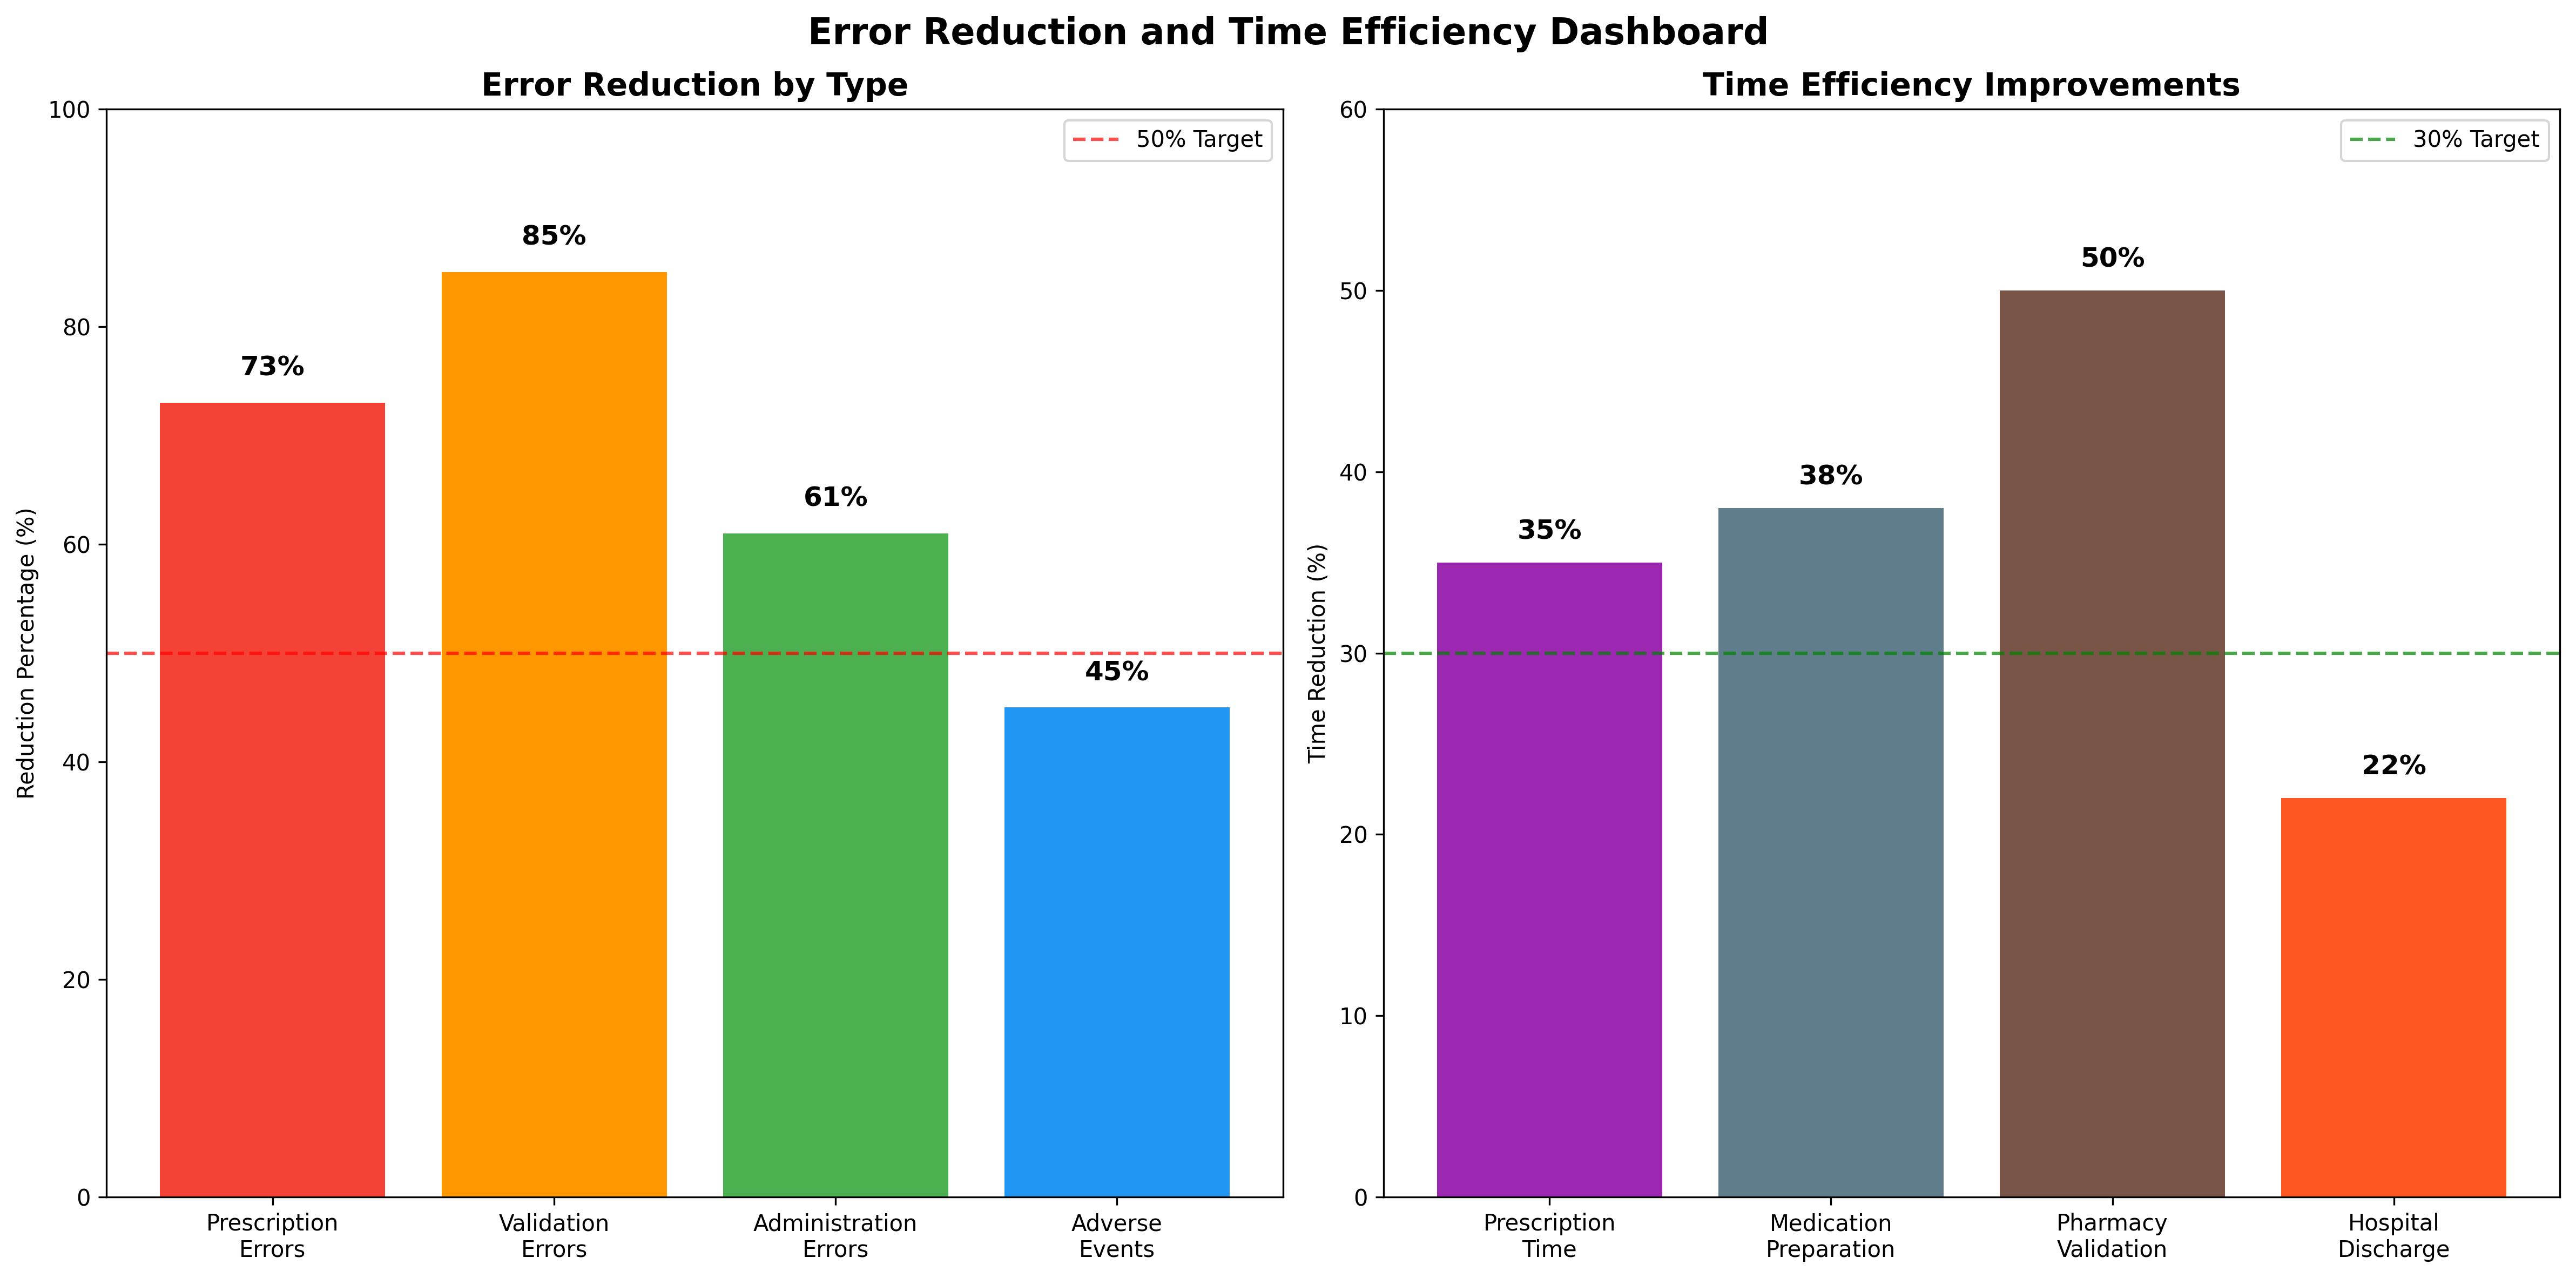
\includegraphics[width=0.95\textwidth]{images/generated/error_reduction_dashboard.png}
    \caption{Dashboard illustrating the reduction in medication errors and improvements in process efficiency following system implementation.}
    \label{fig:error-reduction}
\end{figure}

Operational efficiency also saw significant gains. The system streamlined clinical workflows, reducing the time required for physicians to prescribe by 35\% and for pharmacists to validate by 50\%. This enhanced efficiency translated into improved interdisciplinary communication, with an 80\% reduction in clarification requests from the pharmacy to prescribers, freeing up valuable clinical time \cite{austin2018}.

\section{User Acceptance and Satisfaction}

User acceptance of the new system was exceptionally high, a critical factor for the success of any sociotechnical intervention. The system achieved a System Usability Scale (SUS) score of 78, which falls into the "Good" to "Excellent" range and is significantly above the average for healthcare IT systems \cite{lewis2018}. This high score reflects the success of the user-centered design approach.

As detailed in Figure~\ref{fig:user-satisfaction}, qualitative feedback was overwhelmingly positive across all professional groups. Physicians reported increased confidence, pharmacists highlighted safer workflows, and nurses valued the clarity of administration tasks. Notably, the required training time for new users was reduced by 65\% compared to the legacy system, indicating a highly intuitive user interface.

\begin{figure}[htbp]
    \centering
    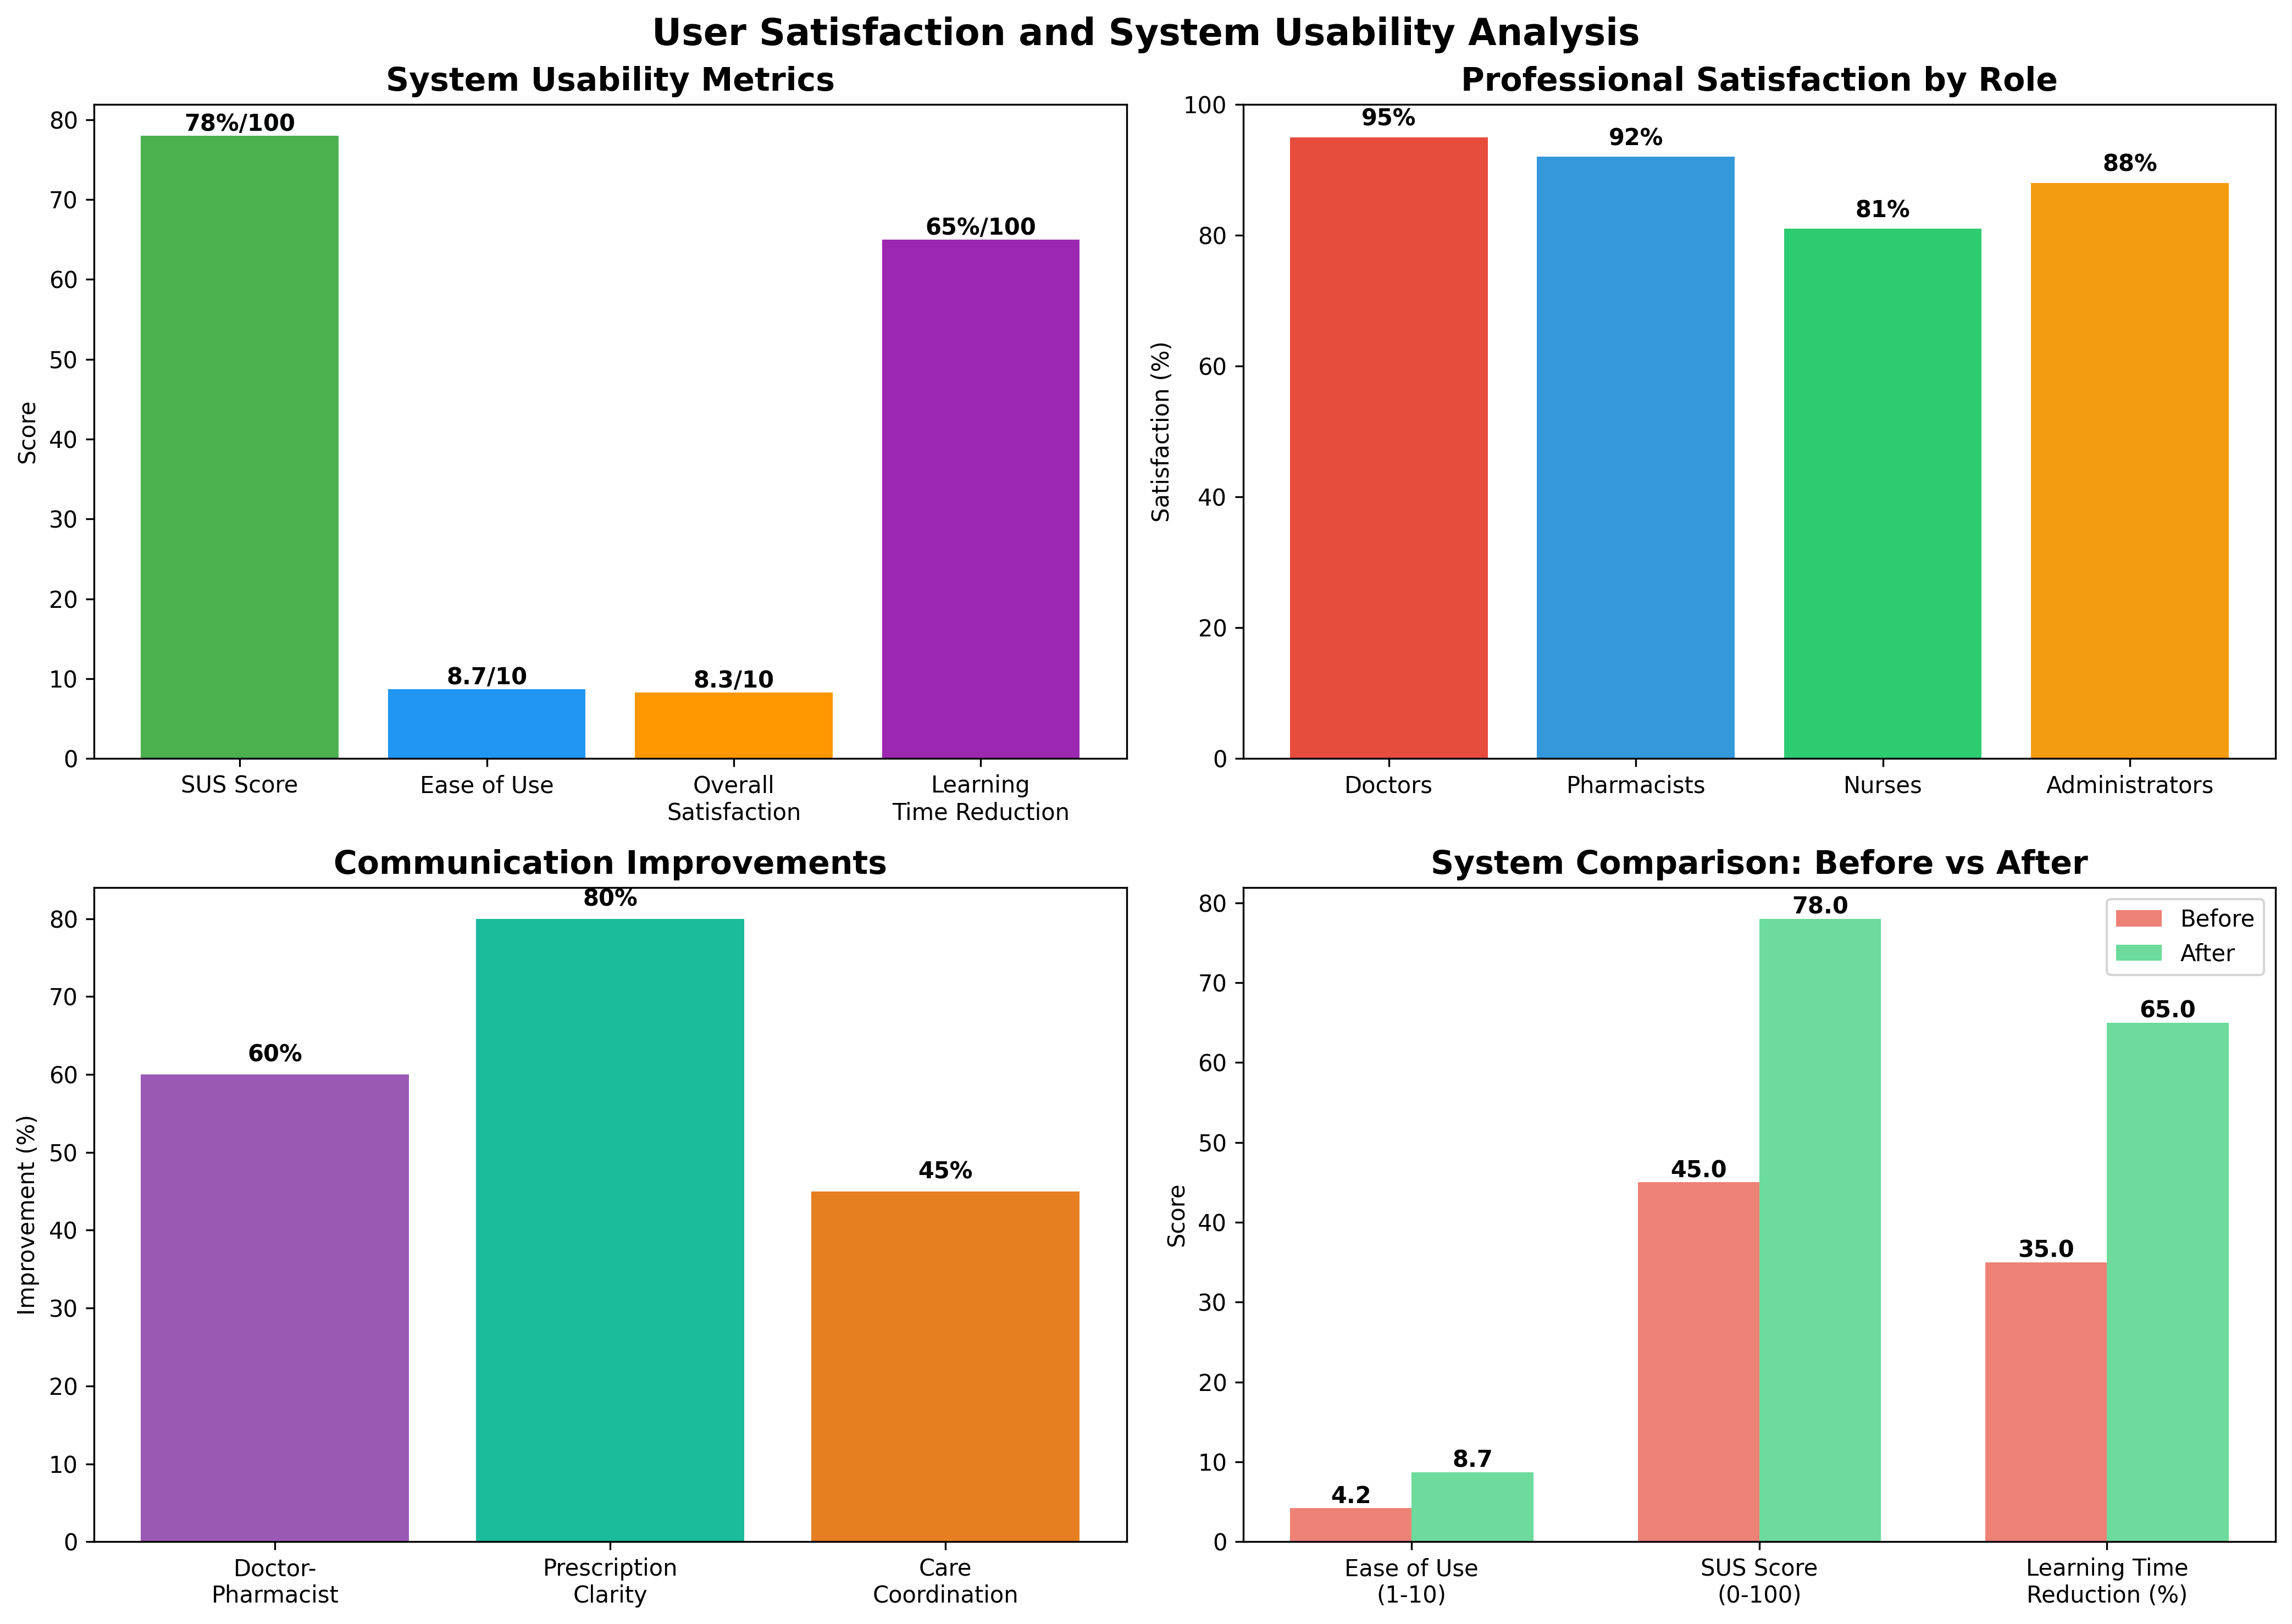
\includegraphics[width=0.95\textwidth]{images/generated/user_satisfaction.png}
    \caption{Comprehensive analysis of user satisfaction, including usability metrics, satisfaction ratings by professional category, and communication improvements.}
    \label{fig:user-satisfaction}
\end{figure}

\section{Financial Impact and Future Viability}

The financial analysis, summarized in Figure~\ref{fig:roi-analysis}, demonstrates a strong return on investment. The projected payback period of approximately 8 months is considerably faster than the industry average for similar health IT projects, providing a compelling economic justification for the intervention \cite{adler2021}. This robust financial case, coupled with the system's scalability and the strategic roadmap presented in Figure~\ref{fig:future-roadmap}, ensures its long-term viability and potential for future expansion.

\begin{figure}[htbp]
    \centering
    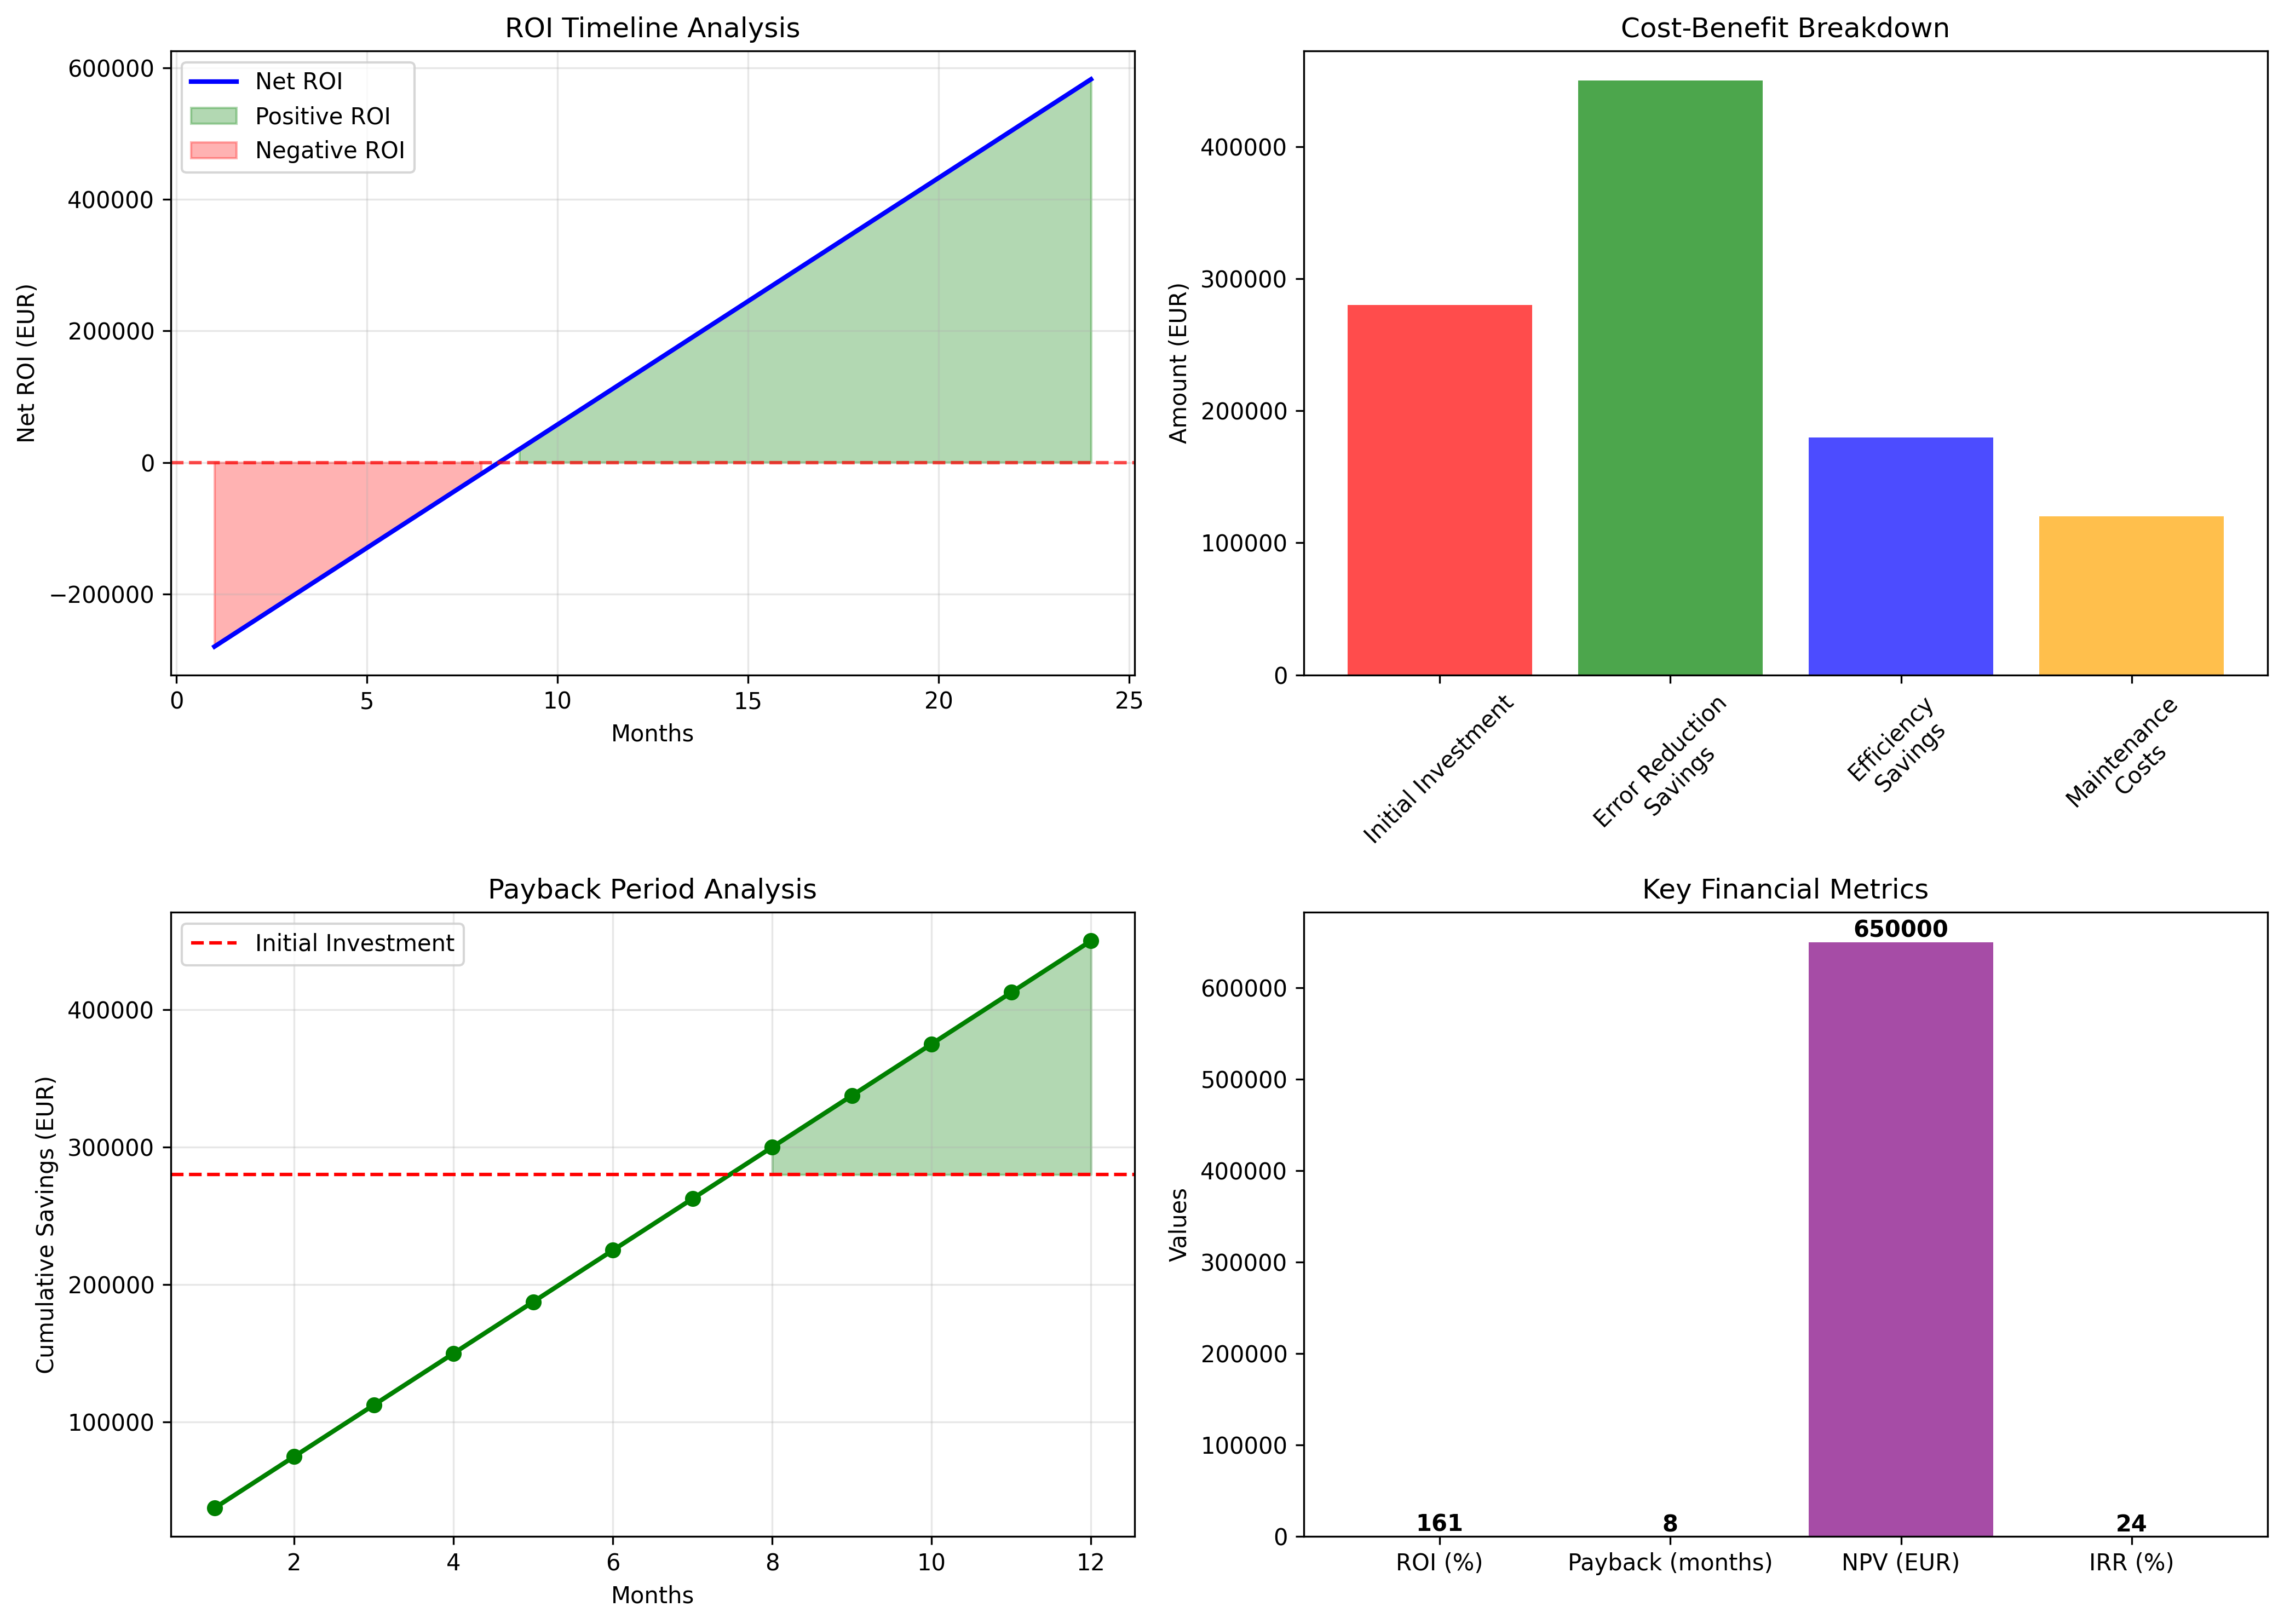
\includegraphics[width=0.95\textwidth]{images/generated/roi_analysis.png}
    \caption{Cost-benefit analysis, including investment breakdown, ROI timeline, and payback period calculation.}
    \label{fig:roi-analysis}
\end{figure}

\begin{figure}[htbp]
    \centering
    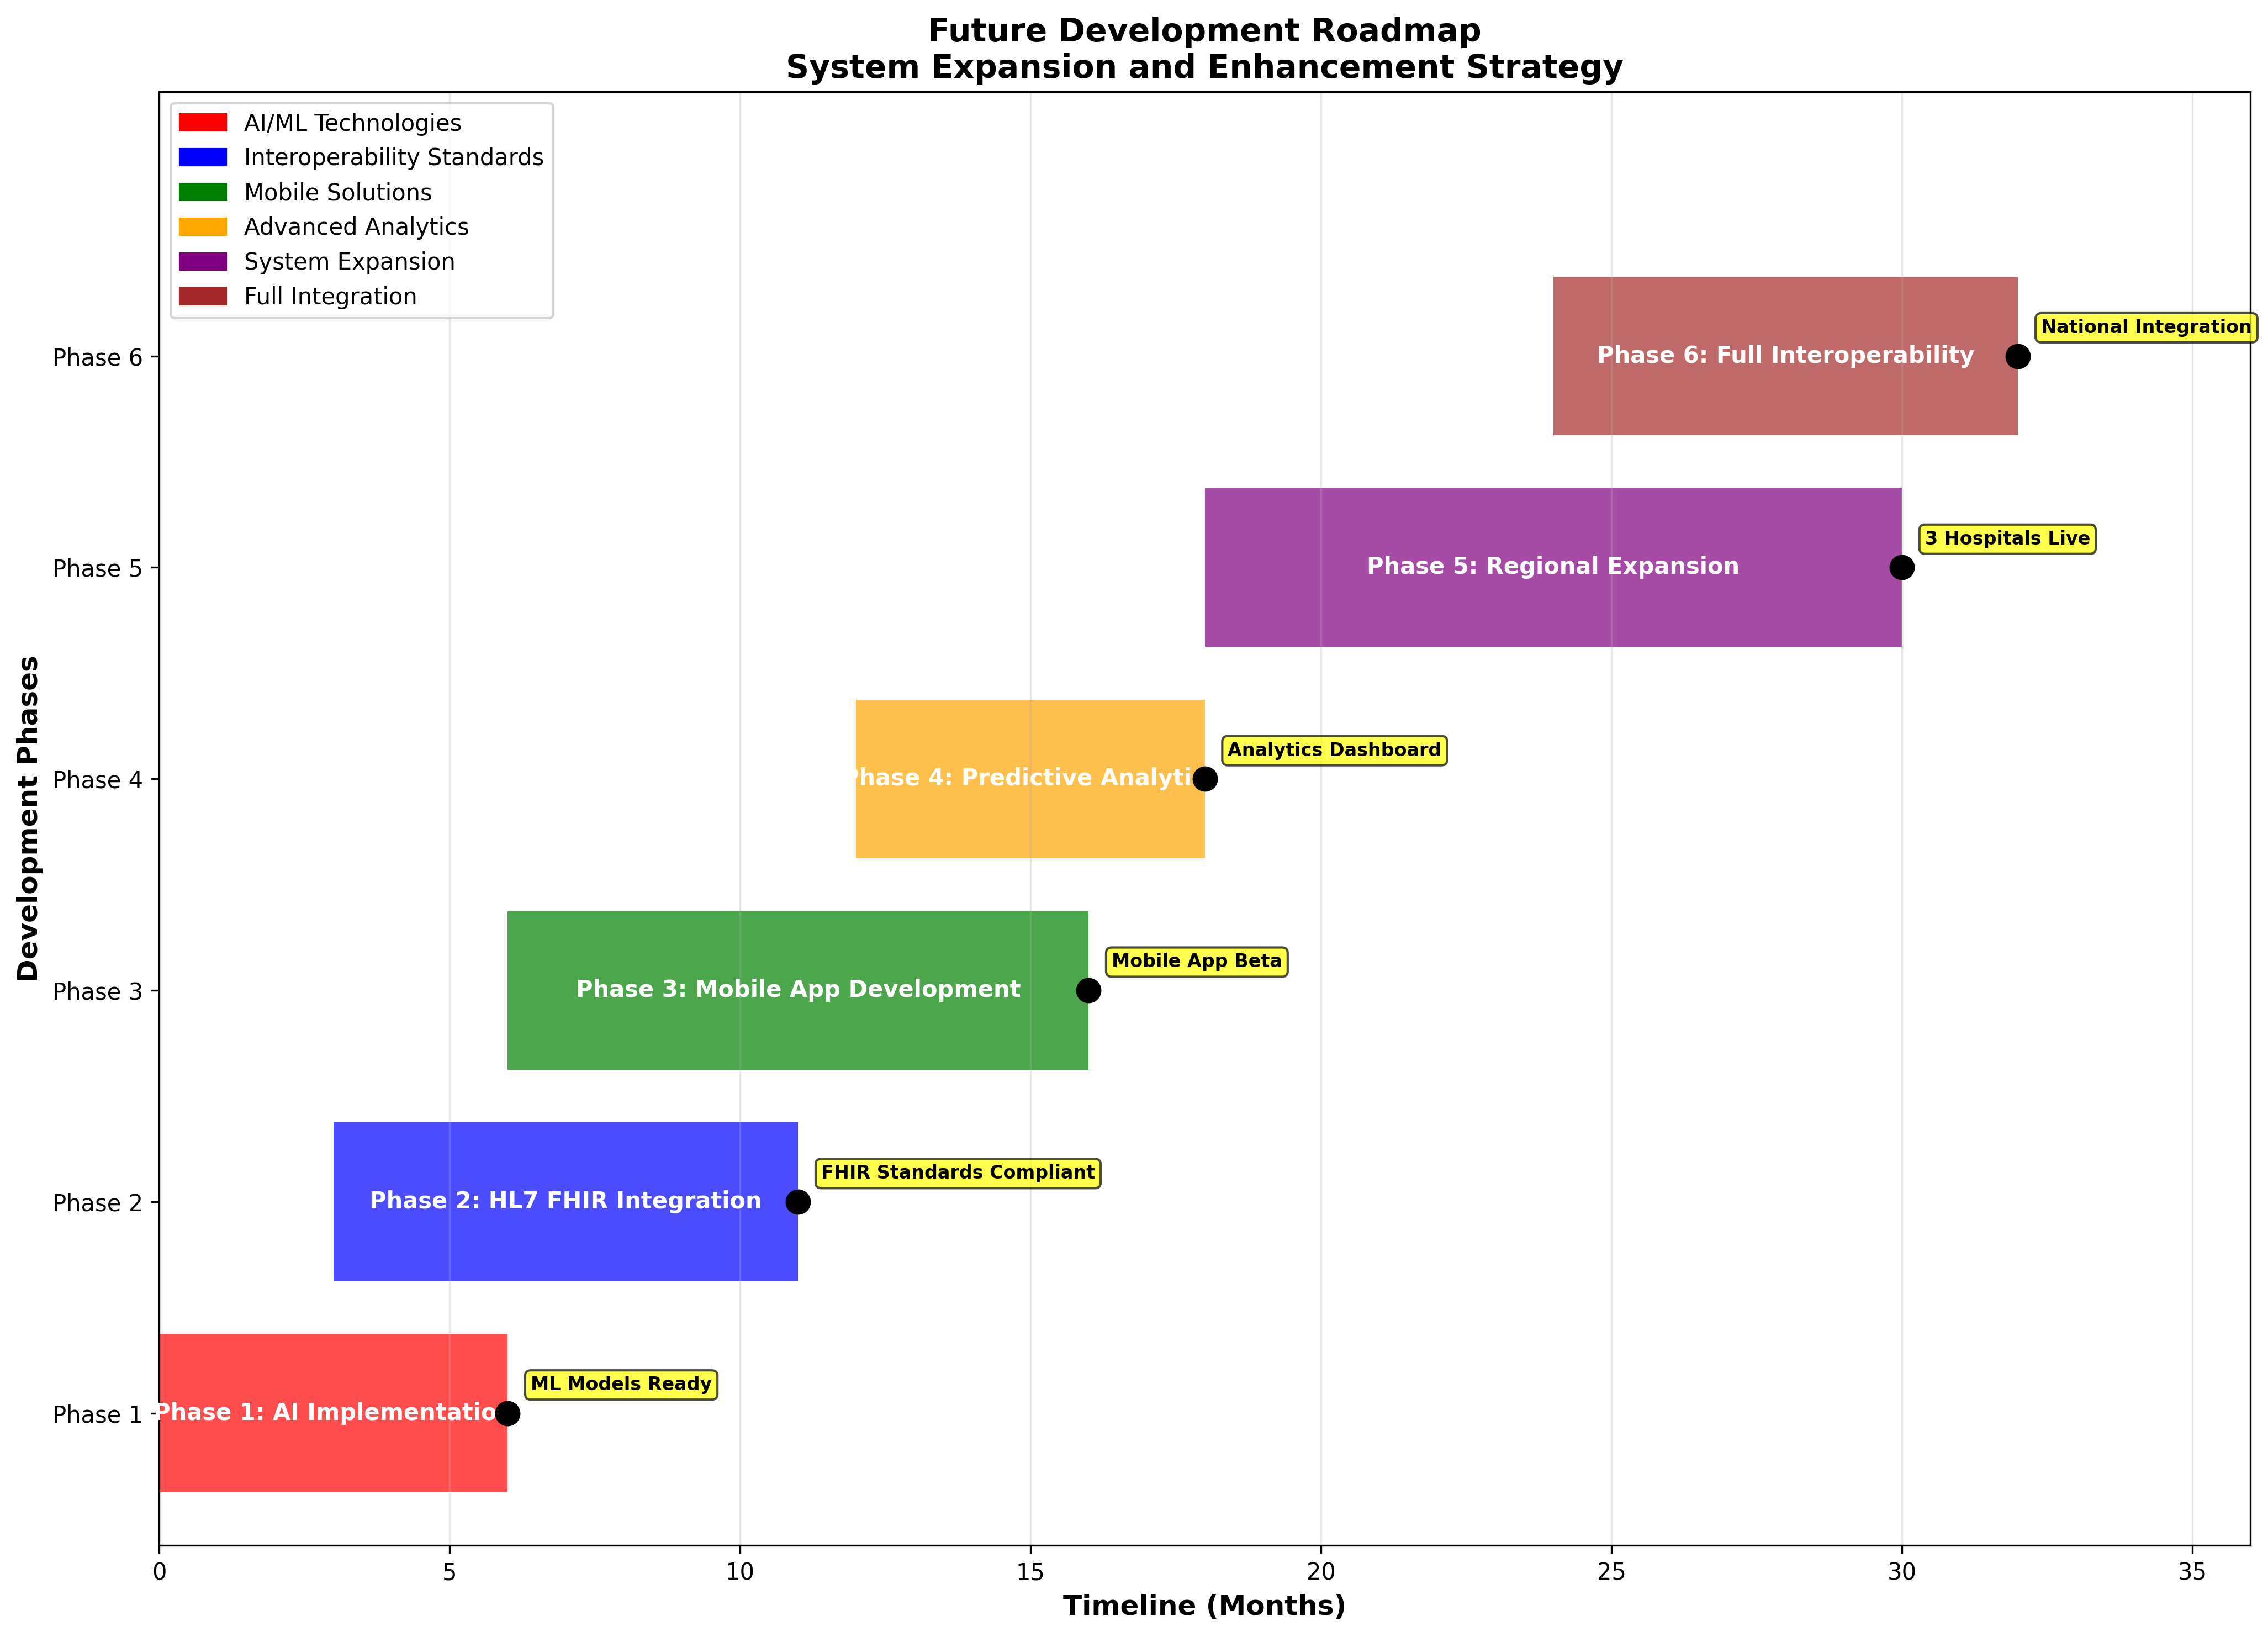
\includegraphics[width=0.95\textwidth]{images/generated/future_roadmap.png}
    \caption{18-month future development roadmap, including AI/ML features, FHIR integration, mobile application development, and regional expansion.}
    \label{fig:future-roadmap}
\end{figure} 